\documentclass[../main.tex]{subfiles}

\begin{document}

\section{Introduction}

\subsection{Bacterial Chemotaxis as a Model System}
The benefits of using model organisms in science are comprehensive. In the field of systems biology, model systems take this central role, and amongst them bacterial chemotaxis in \ecoli is one of the most extensively studied. The stoichiometry is well established\cite{li04}, the structure of many of the constituent proteins have been determined\cite{milligan87, stock89}, and the feedback loops involved described\cite{kentner09} and robustness tested\cite{yi00}. The \ecoli system has also been used as the basis for study of chemotaxis in other bacterium\cite{hamadeh11}.

In more recent times with the advent of more and more powerful computers, chemotaxis in \ecoli has presented itself as an ideal target for the development of advanced simulation packages, allowing researchers to postulate new and more detailed mechanisms of control\cite{lipkow06}. Together with advances in high resolution microscopy\cite{greenfield09} this has opened the door to new insights into the behaviour of the \ecoli chemotaxis network.

The outcome of this research is the following model of chemotaxis:

\begin{figure}[h!]
\begin{center}
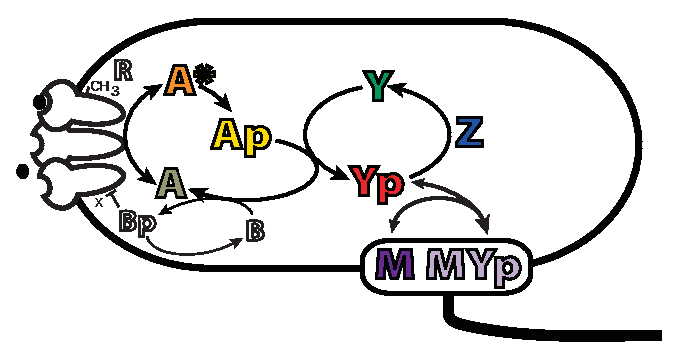
\includegraphics[scale=1]{\docroot introduction/figs/chemotaxis-simple-network}
\caption{Schematic of the chemotaxis system. Note that protein labels are only loosely representative of respective locations in the cell. Figure from Sewitz \& Lipkow\cite{lipkowfigs}.}
\end{center}
\end{figure}

Transmembrane methyl-accepting chemotaxis proteins (MCPs) sit in a cluster at one or both poles of the cell. The presence of repellents or attractants is transduced through a piston like motion\cite{hall11}, with the level of transduction modulated by the level of methylation. The methyltransferase CheR, localised to the MCP, constitutively methylates the MCPs. Phosphorylated methylesterase CheB competes with CheR to demthylate the MCPs. CheB activity is regulated by histidine kinease CheA, whose autophosphorylation is regulated by the activity of the  MCPs. Herein we find the first feedback mechanism, in which an increase in activity causes a decrease in sensitivity.

Phosphrylated CheA also phosphyrlates CheY, a messenger protein which diffuses throughout the cell. Downstream of this there is a bistable-like system which regulates the response of the motors to CheYp, but this is independent of all activity upstream of CheYp. The last significant protein in the \ecoli chemotaxis pathway is the phosphotase CheZ, which removes the phosphate group from CheY.

Despite the extensive coverage of research, there are many areas yet to be fully resolved. Amongst these is that simulations of the system as described above make it apparent that it does not have the same dynamic range as \ecoli do; that is, \ecoli can respond to small changes as well at already high concentrations as low concentrations. Another feedback loop is therefore required to allow the system to retain sensitivity as concentrations change.

Models of the chemotaxis system in which CheZ clusters at the polar clusters in response to changes in CheYp provide this required dynamic range.

\begin{figure}
\begin{center}
\subfigure[Mechanism of clustering]{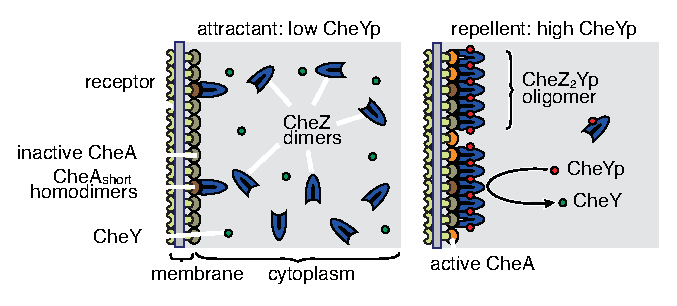
\includegraphics[scale=1]{figs/chezclustering}}\\
\subfigure[Dynamic range improvement]{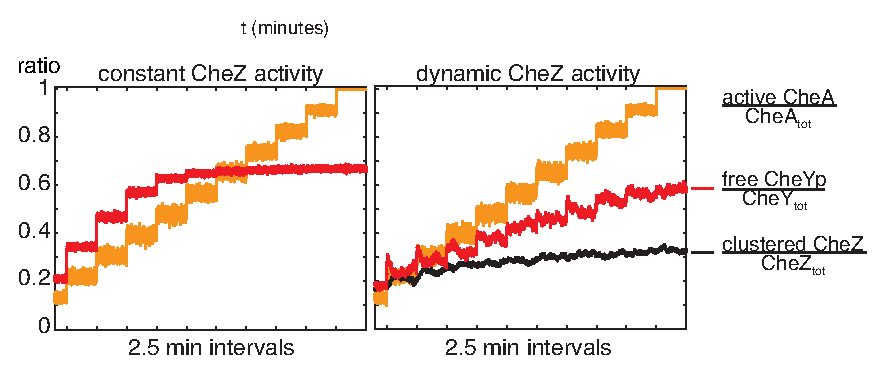
\includegraphics[scale=1]{figs/chezdynamics}}
\caption{stuff}
\end{center}
\end{figure}


This feedback loop is what is covered in the work presented in this report. CheZ forms clusters at the poles of the cells, as well as being found distributed throughout the cytoplasm. Models show that dynamic localisation of CheZ in response to chemotactic activity would increase the dynamic range of the system to match that observed in \ecoli\cite{lipkow06}. To verify this, it is necessary to demonstrate that a greater or lesser proportion of CheZ can be found in the polar clusters while the cell is responding to a chemotactic stimulant.

\subsection{Microscopy}

Microscopy is a rapidly changing field, with advancements coming from all areas. Improvements in optics are yielding diminishing returns in increasing optical resolution, but new illumination and image processing techniques are allowing for finer and finer imaging using otherwise standard equipment, and most manufacturers are now emphasising this area of development more and more in their brochures.

\subsubsection{STORM/PALM super-resolution}
In the context of our challenge - localising proteins and determining density - it would be ideal if we could locate each protein within the \ecoli cell. However, as an \ecoli cell is normally not more than \SI{0.5}{\micro\meter}, and the optical resolution of the microscope is on the order of \SI{200}{\nano\meter}, this is unfeasible using epifluorescent techniques. However, by stochastically illuminating a small arbitrary subset of all the fluorophores over and over and then identifying each fluorescent point as a fluorescently labelled protein it is possible to build up a composite picture of all the proteins. This has already been demonstrated to work for \ecoli chemotaxis proteins.

This stochastic illumination can be achieved in two ways. In STORM\myfootnote{STochastic Optical Reconstruction Microscopy}, a photo-switching fluorophore is required. A weak activation laser is used such that only a few fluorophores at a time are activated; these are then read off by normal excitation illumination. By contrast, in PALM\myfootnote{PhotoActivated Localisation Microscopy} `normal' fluorophores are used but a very powerful bleaching laser forces all but a few of them back to the ground state before they have a chance to fluoresce, achieving the same effect.

PALM requires a relatively powerful bleaching laser, and both require highly sensitive and very fast cameras. They do not require very high resolution optics however, as all that is taken from the optics is the location of a 2D Gaussian. Even so, the higher the resolution the more fluorophores can be imaged simultaneously and the shorter each capture takes. The number of frames required for an image to be built up varies depending on how many fluorophores you are imaging - the more frames the better - but 10,000 is considered to be a reasonable number. Even with some of the fastest cameras available today this would take several seconds.

The image processing techniques required to convert the set of images into a set of locations are not terribly advanced but do require some understanding. Many microscope manufacturers are beginning to offer their own software to do this processing.

\subsubsection{STED Microscopy}

STED\myfootnote{STimulated Emission Depletion} microscopy is an extension of confocal microscopy that improves the resolution from the norm of around \SI{200}{\nano\meter} to, depending on equipment used, less than \SI{10}{\nano\meter}\cite{rittweger09}. A normal confocal illumination source is used, and combined with a doughnut shaped depletion source. The doughnut has an outer radius larger than the illumination source, and an adjustable inner radius less than that of the illumination source. The result is an effective illumination source that is the size of the hole in the doughnut, hence a higher resolution.

\subsubsection{TIRF Microscopy}
As this project is looking at proteins localised near the membrane of the cell, TIRF\myfootnote{Total Internal Reflectance Fluorescence} should have been an ideal technique. By firing a laser at an extremely oblique angle at the sample an evanescent wave is created where the laser reflects inside the coverslip. This extends about \SI{100}{\nano\meter} into the sample, depending on the angle at which the laser is incident. Only fluorophores within this field are activated, removing a lot of background noise.

However, aside from requiring a laser this is also a very tricky technique to set up and does not always give tangible benefits, especially given that the chemotaxis clusters have no particular reason to be located on the underside of the cell.

\subsubsection{FRET Microscopy}
As opposed to STORM/PALM microscopy, which measure the location of fluorophores and then infer the density, it is possible to measure the density of a population directly. FRET\myfootnote{F\"orster Resonance Energy Transfer} is more commonly used to determine the separation of two different fluorophores (Hetero-FRET), but it can also be used to determine the separation of two identical fluorophores (Homo-FRET).

Rather than measuring the conversion of emission from one fluorophore to the emission of another by filtering out different wavelengths as in hetero-FRET, homo-FRET exploits the polarising properties of fluorophores. Fluorophores fluoresce in the same polarisation as they are excited, and they may only be excited by light polarised in alignment with them. FRET, however, is polarisation independent. One fluorophore which is excited by polarised light can transfer its excited state through FRET to a fluorophore which may not be aligned with the polarisation. 

This results in a degree of cross-polarised light being emitted from the sample, which corresponds to the proximity of fluorophores to each other. This technique does not require lasers, but does need monomeric fluorophores that do not spin too fast. If they do, it is likely that they will be excited by the polarised light, but by the time they fluoresce they have spun into a cross-polarised orientation.

\subsection{Objective}
It is the objective of this project to prove whether CheZ dynamically clusters to the pole of \ecoli cells in response to a chemotactic stimulant. This will be measured ultimately using homo-FRET. The stimulant will be an attractant, a repellent, or a simulated stimulant, blue light at \SI{440}{\nano\meter}\cite{wright06}. Levels of chemotactic stimulant will be varied using a microfluidic device.

The primary challenges of this project are threefold:
\begin{enumerate}
\item Design and implement a microscopy set-up for homo-FRET
\item Design and implement a microfluidics set-up for media exchange
\item Design and implement \ecoli strains with the necessary protein fusions
\end{enumerate}

The secondary challenges of this project include
\begin{enumerate}
\item Replicate homo-FRET results for clustering of tar proteins
\item Develop image processing tools for cluster identification
\item Link advanced homo-FRET microscopy techniques to basic epifluorescence techniques
\end{enumerate}
The motivation behind this third point is that if we can demonstrate that simple epifluorescence techniques can also provide the same results as more complex techniques (like homo-FRET), then it will be much easier in the future for other people to work on similar projects.

\end{document}